\documentclass{standalone}
\usepackage{tikz}
\usetikzlibrary{patterns, positioning}


\begin{document}
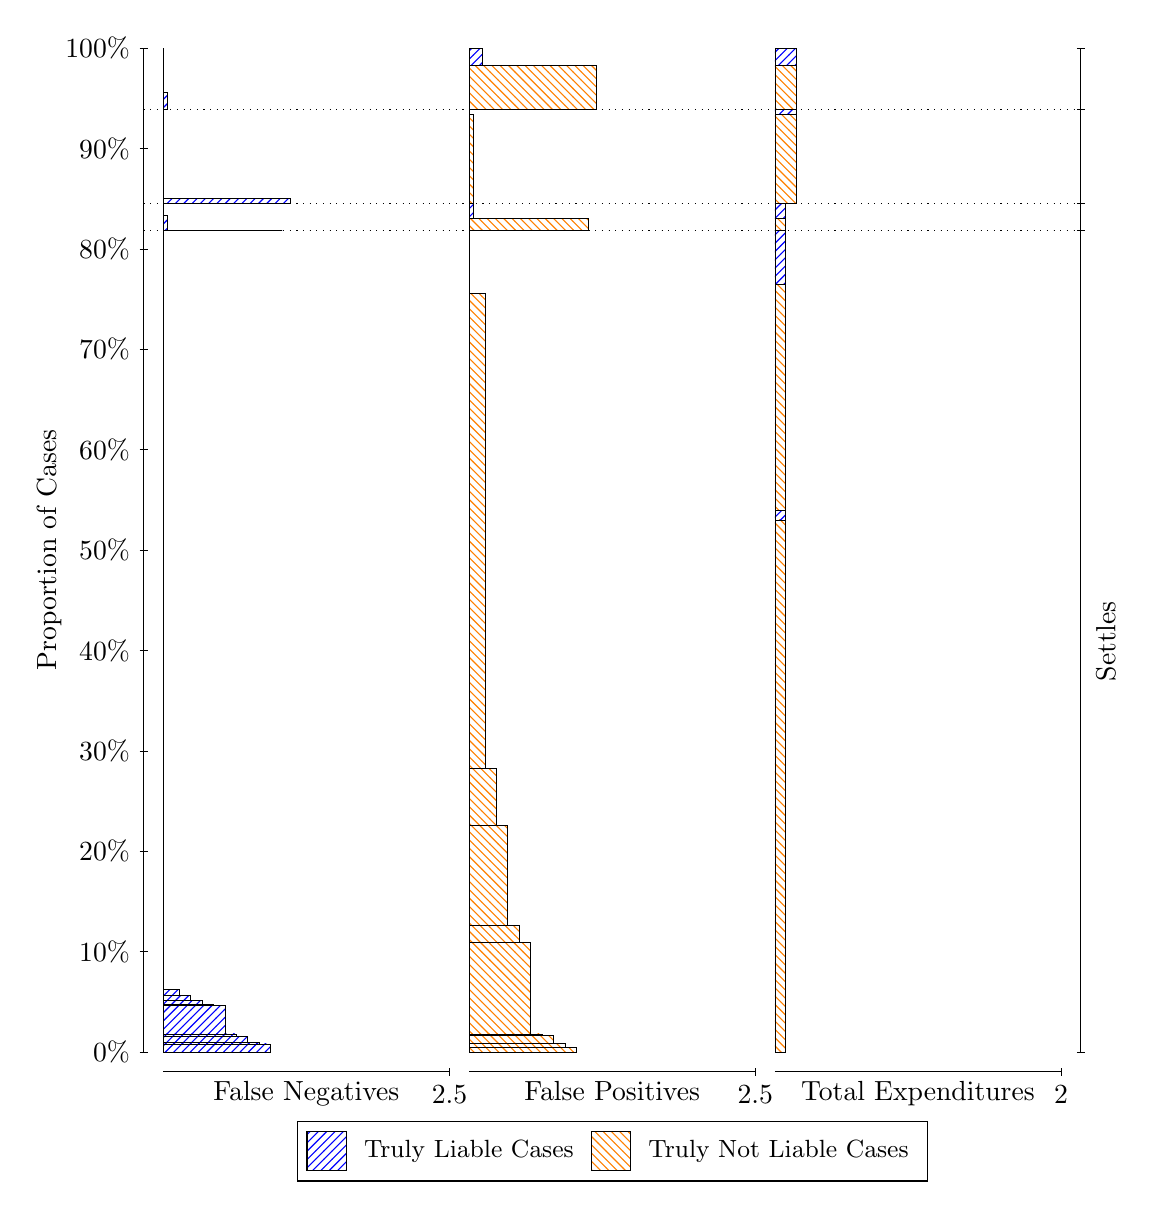
\begin{tikzpicture}
\draw[black, very thin] (1.5,1.75) -- (1.5,14.5);
\node[rotate=90, text=black, anchor=center] at (0.3, 8.125) {Proportion of Cases};
\draw[black, very thin] (1.45,1.75) -- (1.55,1.75);
\node[text=black, anchor=east] at (1.45, 1.75) {0\%};
\draw[black, very thin] (1.45,3.025) -- (1.55,3.025);
\node[text=black, anchor=east] at (1.45, 3.025) {10\%};
\draw[black, very thin] (1.45,4.3) -- (1.55,4.3);
\node[text=black, anchor=east] at (1.45, 4.3) {20\%};
\draw[black, very thin] (1.45,5.575) -- (1.55,5.575);
\node[text=black, anchor=east] at (1.45, 5.575) {30\%};
\draw[black, very thin] (1.45,6.85) -- (1.55,6.85);
\node[text=black, anchor=east] at (1.45, 6.85) {40\%};
\draw[black, very thin] (1.45,8.125) -- (1.55,8.125);
\node[text=black, anchor=east] at (1.45, 8.125) {50\%};
\draw[black, very thin] (1.45,9.4) -- (1.55,9.4);
\node[text=black, anchor=east] at (1.45, 9.4) {60\%};
\draw[black, very thin] (1.45,10.675) -- (1.55,10.675);
\node[text=black, anchor=east] at (1.45, 10.675) {70\%};
\draw[black, very thin] (1.45,11.95) -- (1.55,11.95);
\node[text=black, anchor=east] at (1.45, 11.95) {80\%};
\draw[black, very thin] (1.45,13.225) -- (1.55,13.225);
\node[text=black, anchor=east] at (1.45, 13.225) {90\%};
\draw[black, very thin] (1.45,14.5) -- (1.55,14.5);
\node[text=black, anchor=east] at (1.45, 14.5) {100\%};

\draw[black, very thin] (13.4,1.75) -- (13.4,14.5);
\draw[black, very thin] (13.35,1.75) -- (13.45,1.75);
\node[anchor=west] at (13.35, 1.75) {};
\draw[black, very thin] (13.35,12.183) -- (13.45,12.183);
\node[anchor=west] at (13.35, 12.183) {};
\draw[black, very thin] (13.35,12.188) -- (13.45,12.188);
\node[anchor=west] at (13.35, 12.188) {};
\draw[black, very thin] (13.35,12.526) -- (13.45,12.526);
\node[anchor=west] at (13.35, 12.526) {};
\draw[black, very thin] (13.35,13.716) -- (13.45,13.716);
\node[anchor=west] at (13.35, 13.716) {};
\draw[black, very thin] (13.35,14.5) -- (13.45,14.5);
\node[anchor=west] at (13.35, 14.5) {};

\draw[black, very thin, pattern color=blue, pattern=north east lines] (1.75,1.75) rectangle (3.1125,1.8529);
\draw[black, very thin, pattern color=blue, pattern=north east lines] (1.75,1.8529) rectangle (2.9672,1.8711);
\draw[black, very thin, pattern color=blue, pattern=north east lines] (1.75,1.8711) rectangle (2.8218,1.9497);
\draw[black, very thin, pattern color=blue, pattern=north east lines] (1.75,1.9497) rectangle (2.6765,1.9793);
\draw[black, very thin, pattern color=blue, pattern=north east lines] (1.75,1.9793) rectangle (2.5312,2.3442);
\draw[black, very thin, pattern color=blue, pattern=north east lines] (1.75,2.3442) rectangle (2.3858,2.3561);
\draw[black, very thin, pattern color=blue, pattern=north east lines] (1.75,2.3561) rectangle (2.2405,2.4091);
\draw[black, very thin, pattern color=blue, pattern=north east lines] (1.75,2.4091) rectangle (2.0952,2.4638);
\draw[black, very thin, pattern color=blue, pattern=north east lines] (1.75,2.4638) rectangle (1.9498,2.5495);
\draw[black, very thin, pattern color=orange, pattern=north west lines] (1.75,2.5495) rectangle (1.75,12.183);
\draw[black, very thin, pattern color=blue, pattern=north east lines] (1.75,12.183) rectangle (3.2578,12.183);
\draw[black, very thin, pattern color=orange, pattern=north west lines] (1.75,12.183) rectangle (1.75,12.188);
\draw[black, very thin, pattern color=blue, pattern=north east lines] (1.75,12.188) rectangle (1.8045,12.378);
\draw[black, very thin, pattern color=orange, pattern=north west lines] (1.75,12.378) rectangle (1.75,12.526);
\draw[black, very thin, pattern color=blue, pattern=north east lines] (1.75,12.526) rectangle (3.3668,12.587);
\draw[black, very thin, pattern color=orange, pattern=north west lines] (1.75,12.587) rectangle (1.75,13.716);
\draw[black, very thin, pattern color=blue, pattern=north east lines] (1.75,13.716) rectangle (1.8045,13.939);
\draw[black, very thin, pattern color=orange, pattern=north west lines] (1.75,13.939) rectangle (1.75,14.5);
\draw[black, very thin, pattern color=orange, pattern=north west lines] (5.6333,1.75) rectangle (6.9958,1.8047);
\draw[black, very thin, pattern color=orange, pattern=north west lines] (5.6333,1.8047) rectangle (6.8505,1.8579);
\draw[black, very thin, pattern color=orange, pattern=north west lines] (5.6333,1.8579) rectangle (6.7052,1.9581);
\draw[black, very thin, pattern color=orange, pattern=north west lines] (5.6333,1.9581) rectangle (6.5598,1.9804);
\draw[black, very thin, pattern color=orange, pattern=north west lines] (5.6333,1.9804) rectangle (6.4145,3.1434);
\draw[black, very thin, pattern color=orange, pattern=north west lines] (5.6333,3.1434) rectangle (6.2692,3.3549);
\draw[black, very thin, pattern color=orange, pattern=north west lines] (5.6333,3.3549) rectangle (6.1238,4.6249);
\draw[black, very thin, pattern color=orange, pattern=north west lines] (5.6333,4.6249) rectangle (5.9785,5.3529);
\draw[black, very thin, pattern color=orange, pattern=north west lines] (5.6333,5.3529) rectangle (5.8332,11.383);
\draw[black, very thin, pattern color=blue, pattern=north east lines] (5.6333,11.383) rectangle (5.6333,12.183);
\draw[black, very thin, pattern color=orange, pattern=north west lines] (5.6333,12.183) rectangle (5.6878,12.188);
\draw[black, very thin, pattern color=blue, pattern=north east lines] (5.6333,12.188) rectangle (5.6333,12.188);
\draw[black, very thin, pattern color=orange, pattern=north west lines] (5.6333,12.188) rectangle (7.1412,12.335);
\draw[black, very thin, pattern color=blue, pattern=north east lines] (5.6333,12.335) rectangle (5.6878,12.526);
\draw[black, very thin, pattern color=orange, pattern=north west lines] (5.6333,12.526) rectangle (5.6878,13.654);
\draw[black, very thin, pattern color=blue, pattern=north east lines] (5.6333,13.654) rectangle (5.6333,13.716);
\draw[black, very thin, pattern color=orange, pattern=north west lines] (5.6333,13.716) rectangle (7.2502,14.277);
\draw[black, very thin, pattern color=blue, pattern=north east lines] (5.6333,14.277) rectangle (5.7968,14.5);
\draw[black, very thin, pattern color=orange, pattern=north west lines] (9.5167,1.75) rectangle (9.6529,8.5083);
\draw[black, very thin, pattern color=blue, pattern=north east lines] (9.5167,8.5083) rectangle (9.6529,8.6294);
\draw[black, very thin, pattern color=orange, pattern=north west lines] (9.5167,8.6294) rectangle (9.6529,11.504);
\draw[black, very thin, pattern color=blue, pattern=north east lines] (9.5167,11.504) rectangle (9.6529,12.183);
\draw[black, very thin, pattern color=orange, pattern=north west lines] (9.5167,12.183) rectangle (9.6529,12.188);
\draw[black, very thin, pattern color=blue, pattern=north east lines] (9.5167,12.188) rectangle (9.6529,12.188);
\draw[black, very thin, pattern color=orange, pattern=north west lines] (9.5167,12.188) rectangle (9.6529,12.335);
\draw[black, very thin, pattern color=blue, pattern=north east lines] (9.5167,12.335) rectangle (9.6529,12.526);
\draw[black, very thin, pattern color=orange, pattern=north west lines] (9.5167,12.526) rectangle (9.7892,13.654);
\draw[black, very thin, pattern color=blue, pattern=north east lines] (9.5167,13.654) rectangle (9.7892,13.716);
\draw[black, very thin, pattern color=orange, pattern=north west lines] (9.5167,13.716) rectangle (9.7892,14.277);
\draw[black, very thin, pattern color=blue, pattern=north east lines] (9.5167,14.277) rectangle (9.7892,14.5);
\draw[black, dotted] (1.5,12.183) -- (13.4,12.183);
\draw[black, dotted] (1.5,12.188) -- (13.4,12.188);
\draw[black, dotted] (1.5,12.526) -- (13.4,12.526);
\draw[black, dotted] (1.5,13.716) -- (13.4,13.716);
\draw[black, very thin] (1.75,1.5) -- (5.3833,1.5);
\node[text=black, anchor=north] at (3.5667, 1.5) {False Negatives};
\draw[black, very thin] (5.3833,1.45) -- (5.3833,1.55);
\node[text=black, anchor=north] at (5.3833, 1.45) {2.5};

\draw[black, very thin] (5.6333,1.5) -- (9.2667,1.5);
\node[text=black, anchor=north] at (7.45, 1.5) {False Positives};
\draw[black, very thin] (9.2667,1.45) -- (9.2667,1.55);
\node[text=black, anchor=north] at (9.2667, 1.45) {2.5};

\draw[black, very thin] (9.5167,1.5) -- (13.15,1.5);
\node[text=black, anchor=north] at (11.333, 1.5) {Total Expenditures};
\draw[black, very thin] (13.15,1.45) -- (13.15,1.55);
\node[text=black, anchor=north] at (13.15, 1.45) {2};

\node[text=black, centered, rotate=90] at (13.72, 6.9663) {Settles};





\draw (7.449999999999999,1.5) node[draw=none] (baseCoordinate) {};
\begin{scope}[align=center]
        \matrix[scale=0.5, draw=black, below=0.5cm of baseCoordinate, nodes={draw}, column sep=0.1cm]{
            \node[rectangle, draw, minimum width=0.5cm, minimum height=0.5cm, pattern color=blue, pattern=north east lines] {}; &
            \node[draw=none, font=\small, text=black] (B) {Truly Liable Cases}; &
            \node[rectangle, draw, minimum width=0.5cm, minimum height=0.5cm, pattern color=orange, pattern=north west lines] {}; &
            \node[draw=none, font=\small, text=black] (B) {Truly Not Liable Cases}; \\
            };
\end{scope}

\end{tikzpicture}
\end{document}